%-------------------------------------------------------------------------------
% Preamble
%-------------------------------------------------------------------------------

\documentclass{article}


%Packages
\usepackage{
	siunitx, % units
	cleveref,% cross-references
	physics, % better physics notation
	url, % for URLs
	amsmath, % for math
	array, % for fixed-width tables
  graphicx, % for images
}

\usepackage[letterpaper]{geometry}
\renewcommand{\thefigure}{S\arabic{figure}}

%-------------------------------------------------------------------------------
% Title and Authors
%-------------------------------------------------------------------------------

\title{Supplemental Information for\\``Extreme rainfall in Paraguay during the 2015-2016 austral summer: causes and subseasonal-to-seasonal predictive skill''}
\author{James Doss-Gollin\and \'{A}ngel G. Mu\~{n}oz \and Simon J. Mason \and Max Past\'{e}n}
\date{\today}

\begin{document}

%% Necessary!
\maketitle

This document contains several supplemental figures described in the main text.
Further supporting information is available in the form of source code and \texttt{jupyter} notebooks at \url{github.com/jdossgollin/PYFloods}.
\listoffigures
\clearpage

\begin{figure}
	\includegraphics[width=\textwidth]{../_figs/Climatology.pdf}
	\caption{
		NDJF monthly circulation climatology over the study domain and from 1980 to 2010.
    First row shows the \SI{850}{\hecto\pascal} streamfunction $\psi$ climatology, and second row shows rainfall climatology.
	}
\end{figure}

\begin{figure}
  \includegraphics[width=\textwidth]{../_figs/PSI_Var_Explained.pdf}
	\caption{
		Variance explained for each EOF loading of the \SI{850}{\hecto\pascal} streamfunction $\psi$.
    Left figure shows the individual variance explained for each EOF and right figure shows cumulative variance explained.
	}
\end{figure}

\begin{figure}
  \includegraphics[width=\textwidth]{../_figs/WT_Classifiability.pdf}
	\caption{
		Classifiability index (see Methods) calculated for several chosen values of $k$, representing the number of weather types used for clustering.
	}
\end{figure}

\begin{figure}
  \includegraphics[width=\textwidth]{../_figs/WT_Occurrence_Proportion.pdf}
	\caption{
		Occurrence fraction of NDJF weather types for all years (blue) and 2015-16 (orange).
	}
\end{figure}

\begin{figure}
  \includegraphics[width=\textwidth]{../_figs/ENSO_EOF_Scatter.pdf}
	\caption{
		Pair plots for three time series: NINO3.4, and EOFs 2 and 3 of the \SI{850}{\hecto\pascal} field over the chosen domain.
    All time series are degraded to monthly time steps.
    Across the diagonal, marginal distributions are shown.
    Straight lines represent linear regression estimates.
	}
\end{figure}

\begin{figure}
  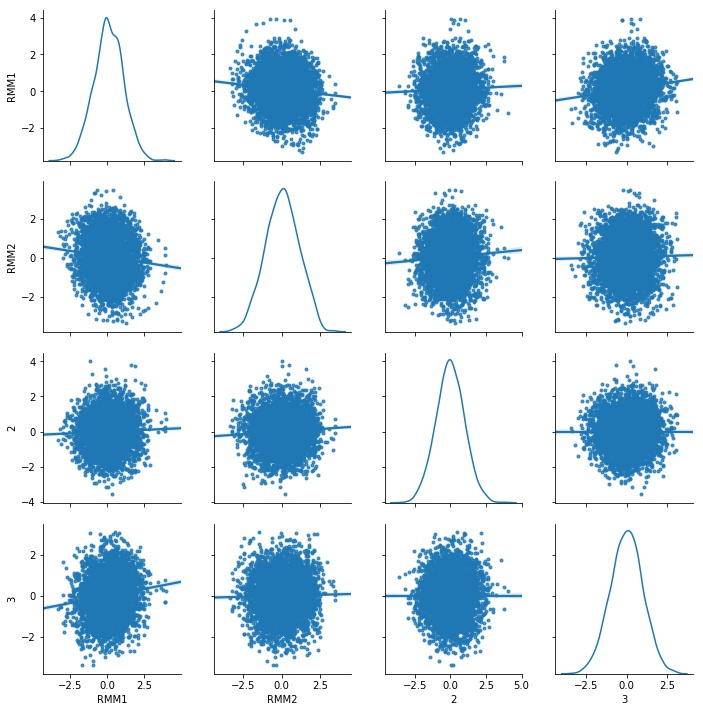
\includegraphics[width=\textwidth]{../_figs/MJO_EOF_Scatter}
	\caption{
		Pair plots for four time series: MJO RMM1 and RMM2, and EOFs 2 and 3 of the \SI{850}{\hecto\pascal} field over the chosen domain.
    All time series are at daily time steps.
    Across the diagonal, marginal distributions are shown.
    Straight lines represent linear regression estimates.
	}
\end{figure}

\begin{figure}
  \includegraphics[width=\textwidth]{../_figs/knn_rainfall_EOF.pdf}
	\caption{
    Expected rainfall over two regions conditional on the (simultaneous) values of EOF2 and EOF3 of the \SI{850}{\hecto\pascal} streamfunction $\psi$ shown in the main text.
    The ``Chaco Jet Extension Region'' is defined as extending from \SIrange{299.25}{302.75}{\degree E} and \SIrange{34.75}{30.75}{\degree S} and the ``Lower Paraguay River Basin'' is defined in the main text.
    Both values represent area-averaged rainfall time series.
    Expected rainfall is calculated by using a nearest-neighbors regression with 100 neighbors.
    Because this methodology performs poorly under extrapolation (where there are few observations), the predicted domain is limited to include only regions with high density of observations.
    }
\end{figure}

\begin{figure}
  \includegraphics[width=\textwidth]{../_figs/ENSO_MJO_EOF_PRCP_Time_Series.pdf}
	\caption{
		Time series of S2S predictors and their influence on evolution of circulation and rainfall.
    Top row shows two predictors shown to influence the circulation: monthly NINO3.4 index and daily MJO RMM1 index.
    Blue dots show daily observations of MJO RMM1, while the blue line shows the MJO RMM1 time series with a 7-day rolling mean applied.
    Bottom row shows the evolution of EOFS 2 and 3 of the \SI{850}{\hecto\pascal} field.
    As for the MJO RMM1, dots show the daily fields and lines show the fields with a 7-day running mean applied.
    Bottom rain shows time series of daily rainfall over the ``Lower Paraguay River Basin'' and ``Chaco Jet Extension Region'' defined above.
	}
\end{figure}

\end{document}
